% Load before IEEEtran to avoid XeTeX TU/Times font substitutions.
\RequirePackage[T1]{fontenc}
\documentclass[conference,a4paper]{IEEEtran}
\IEEEoverridecommandlockouts

% Packages retained from the manuscript; duplicate/conflicting imports removed.
\usepackage{cite}
\usepackage{float}
\usepackage{amsmath,amssymb,amsfonts}
\usepackage{mathtools}
\usepackage{algorithm}
\usepackage{algpseudocode}
\usepackage{graphicx}
\usepackage{textcomp}
\usepackage{xcolor}
\usepackage{booktabs}
\usepackage{tabularx}
\usepackage{array}
\usepackage{nicematrix}
\usepackage{balance}
\usepackage{enumitem}
\usepackage{tikz}
\usepackage{bm}
\usepackage{lipsum}
\usetikzlibrary{shapes.geometric}
\usepackage[hidelinks]{hyperref}

\algrenewcommand\algorithmicrequire{\textbf{Input:}}
\algrenewcommand\algorithmicensure{\textbf{Output:}}
\newtheorem{coro}{Corollary}
\newtheorem{theo}{Theorem}
\newtheorem{prop}{Proposition}
\newtheorem{remark}{Remark}
\newtheorem{example}{Example}
\newtheorem{lemma}{Lemma}
\newtheorem{defin}{Definition}
\hypersetup{breaklinks=true,citecolor=black,colorlinks=true,
            linkcolor=black,urlcolor=blue}
\setcounter{MaxMatrixCols}{30}

\title{Mobility-Aware UAV Positioning and Secret Key Rate Optimization for HAP--UAV CV-QKD}
\author{\IEEEauthorblockN{TBD\IEEEauthorrefmark{1},
TBD\IEEEauthorrefmark{2}}
\IEEEauthorblockA{\IEEEauthorrefmark{1}XXX}
\IEEEauthorblockA{\IEEEauthorrefmark{2}Computer Communications Laboratory,
The University of Aizu, Aizuwakamatsu 965-8580, Japan}}


\begin{document}
\maketitle
\begin{abstract}
This provisional internal-review study examines source selection and UAV positioning for a cloud-affected HAP--UAV discrete-modulated CV-QKD model. A finite catalog of 233 exact-source ensembles defines a common location-dependent numerical rate map. An offline stationary benchmark, a current-slot Greedy policy, and finite-horizon dynamic programming (DP) are compared under identical cloud realizations and speed constraints. Across 100 paired missions, expanding the candidate set from 10 to 100 raises the mean DP penalized objective by 11.41\%. At blockage probability 0.8, mean zero-rate unavailability is 24.60\%, 16.53\%, and 4.07\% for Stationary, Greedy, and DP, respectively. At the representative penalty, DP reduces travel by 88.37\% relative to zero penalty while reducing mean usable rate by 0.515\%. These are conditional manuscript-model outputs: the recorded two-dimensional mutual information and homodyne Holevo expression do not specify a consistent Bob measurement. The results characterize the saved numerical optimization and do not establish physical quantum security.
\end{abstract}
\begin{IEEEkeywords}
Continuous-variable quantum key distribution, UAV, high-altitude platform, cloud blockage, probabilistic shaping, dynamic programming.
\end{IEEEkeywords}
\noindent\textbf{Internal review only.} Security-model correction and author review remain pending. Status:\\
{\footnotesize\texttt{UNVALIDATED\_SECURITY\_MODEL};}\\
{\footnotesize\texttt{NOT\_READY\_FOR\_PUBLICATION\_SCALE\_RUNS}.}
\section{HAP--UAV CV-QKD System and Problem Formulation}
\label{sec:system}
\subsection{Mobility-Aware UAV Positioning and SKR Optimization}
We consider one UAV at a fixed altitude over a $1\,\mathrm{km}\times
1\,\mathrm{km}$ area, discretized into $J$ candidate positions
$\mathcal Q=\{\mathbf q_j\}_{j=1}^J$. The mission has $N_t$ slots of
duration $\Delta t$. Let $c_{j,n}\in\{0,1\}$ indicate cloud blockage
(one means blocked). The matrix $\mathbf C=[c_{j,n}]$ contains spatially
and temporally correlated Bernoulli states. P2 and P3 know the complete
matrix and are offline benchmarks; Greedy observes only the current slot.

For an unblocked link, the recorded manuscript-style raw rate is
\begin{equation}
 K_j(\nu,V_A)=\beta_{\rm rec}I_{AB,j}^{2D}(\nu,V_A)-\chi_{BE,j}(\nu,V_A).
 \label{eq:raw}
\end{equation}
Equation~\eqref{eq:raw} is retained as a conditional numerical metric,
subject to the measurement-consistency limitations below.

\subsection{Recorded Physical-Layer Model and Security Boundary}
\label{sec:security}
Alice sends the coherent-state ensemble $\{p_k,\alpha_k\}_{k=1}^{256}$.
With $[\hat x,\hat p]=2i$ and vacuum quadrature variance one, the
normalization is $V_A=2\sum_kp_k|\alpha_k|^2=2\bar n$.
The source moments $C_s,w_s$ are computed from this same ensemble;
the subscript distinguishes them from the cloud matrix.
For clear-sky power transmittance $\eta$, the saved evaluator uses
\begin{align*}
 \eta_f&=\langle\sqrt\eta\rangle^2,\\
 N=\eta_f\xi_f&=(\langle\eta\rangle-\eta_f)V_A
                  +\xi_{\rm ch}\langle\eta\rangle,\\
 V&=1+V_A,\qquad W=1+\eta_fV_A+N,\\
 Z&=2\sqrt{\eta_f}C_s-\sqrt{2Nw_s}.
\end{align*}
The convention is $\xi_n=\xi_{\rm ch}$. The additive $N$ is
output-referred excess noise; loss-induced vacuum is already included
in $W$'s unit baseline. The active detector is ideal (efficiency one,
electronic noise zero). No imperfect trusted-detector claim is made.
The clear-sky distribution retains a separate angle-of-arrival outage
atom at $\eta=0$ and its active density on $[0,1]$, without renormalizing.
Moment reduction at the covariance level has a precedent for Gaussian
modulation~\cite{usenko2012}; it is not an identity for the full
discrete-input fading likelihood.

Specifically, the saved MI kernel uses the normalized likelihood
\[
 p_{\rm num}(\mathbf y|k)=\frac{
 \exp[-\|\mathbf y-2\sqrt{\eta_f}(\Re\alpha_k,\Im\alpha_k)\|^2/
                 (2(1+N))]}{2\pi(1+N)}
\]
and integrates both real components to obtain $I_{AB}^{2D}$.
The Holevo branch uses the standard-form covariance with entries
$V,W,Z$ and the \emph{homodyne} conditional eigenvalue
\[
 \nu_3^{\rm hom}=\sqrt{V(V-Z^2/W)}.
\]
These two branches do not specify one consistent single-mode Bob
measurement: a homodyne outcome has one quadrature, while joint
measurement of both quadratures adds measurement vacuum. The
measurement-dependent Holevo expressions are explicitly different
in~\cite{denys2021}. Consequently, all reported ``usable SKR'' values
are conditional outputs of the recorded manuscript model, not
established achievable secret-key rates.

Further, evaluating only $Z_-$ does not establish the worst-case
Holevo value over all admissible correlations; the general
interval-maximization caveat in~\cite[Sec.~4, footnotes 11--12]{denys2021}
also applies. A consistent measurement/noise specification, admissible
correlation treatment, parameter estimation, and fading/outage
conditioning protocol require author review. No correction is applied
to the historical numerical results in this manuscript revision.


% Only Optimization through Conclusion is revised; the protected prefix is unchanged.
\typeout{GLOBECOM_LAYOUT textheight=\the\textheight;columnwidth=\the\columnwidth;textwidth=\the\textwidth;topmargin=\the\topmargin;headheight=\the\headheight;headsep=\the\headsep;voffset=\the\voffset}
\raggedbottom
\section{Joint Source and Mobility Optimization}
\label{sec:optimization}
Cloud blockage favors spatial adaptation, but UAV motion incurs travel
cost. We jointly consider source selection, stationary deployment, and
mobility-aware positioning.
The finite catalog $\mathcal G=\{(\nu,V_A)\}$ contains 197 MB-shaped and
36 uniform 256-QAM ensembles. Source selection is
\begin{equation}
 \mathcal P_1:\quad K_j^\star=
 \left[\max_{(\nu,V_A)\in\mathcal G}K_j(\nu,V_A)\right]^+.
 \label{eq:p1}
\end{equation}
Each candidate uses its own exact source moments and fading noise.
Maximize raw rate before clipping; optimality is finite-catalog.
With $S_{j,n}=(1-c_{j,n})K_j^\star$, the best fixed position is
\begin{equation}
 \mathcal P_2:\quad j_{\rm fix}^\star=
 \arg\max_j\frac{1}{N_t}\sum_{n=1}^{N_t}S_{j,n}.
 \label{eq:p2}
\end{equation}
For a trajectory $j_n\in\{1,\ldots,J\}$, define
$d_{i,j}=\|\mathbf q_i-\mathbf q_j\|_2$. The mobility problem is
\begin{align}
 \mathcal P_3:\quad\max_{\{j_n\}}\quad&
 \frac{1}{N_t}\sum_{n=1}^{N_t}S_{j_n,n}
 -\frac{\lambda}{D_{\rm ref}}\sum_{n=2}^{N_t}d_{j_{n-1},j_n}
 \label{eq:p3}\\
 \mathrm{s.t.}\quad&d_{j_{n-1},j_n}\le v_{\max}\Delta t,
                  \quad n=2,\ldots,N_t.\nonumber
\end{align}
Here $U=\overline K-\lambda D/D_{\rm ref}$ balances mean usable rate
$\overline K$ and total distance $D$; $\lambda\ge0$ is in bit/use and
$D_{\rm ref}>0$ normalizes distance. Staying and free initial placement
are allowed, with no deployment or return cost. Distance is a cost
surrogate, not calibrated propulsion energy.

\section{Proposed Solution}
\label{sec:method}
P1 exhausts the catalog once per clear-sky position; P2 compares all $J$
mission means. Let $\mathcal N(j)=\{i:d_{i,j}\le v_{\max}\Delta t\}$,
including staying. Greedy starts at
$j_1^{\rm G}\in\arg\max_jS_{j,1}$ and then selects
\begin{equation}
 j_n^{\rm G}\in\arg\max_{j\in\mathcal N(j_{n-1}^{\rm G})}
 \left[S_{j,n}-\frac{N_t\lambda}{D_{\rm ref}}d_{j_{n-1}^{\rm G},j}\right].
 \label{eq:greedy}
\end{equation}
This $O(N_tJ)$ policy observes the current slot only. DP instead retains
the best prefix ending at each position:
\begin{align}
 F_1(j)&=S_{j,1},\label{eq:dp_init}\\
 F_n(j)&=S_{j,n}+\max_{i\in\mathcal N(j)}
 \left[F_{n-1}(i)-\frac{N_t\lambda}{D_{\rm ref}}d_{i,j}\right].
 \label{eq:dp}
\end{align}
Store maximizing predecessors, choose the best terminal state, and
backtrack. Then
$U^\star=\max_jF_{N_t}(j)/N_t$ in dense worst-case time $O(N_tJ^2)$,
with $O(N_tJ)$ backpointers and an $O(J^2)$ distance matrix.
P2 and DP know the complete cloud sequence offline. DP has no smaller
$U$ than P2 or Greedy, but need not dominate unpenalized rate or availability.
Its advantage also includes future information and initial-position selection.

\begin{figure*}[!t]
\centering
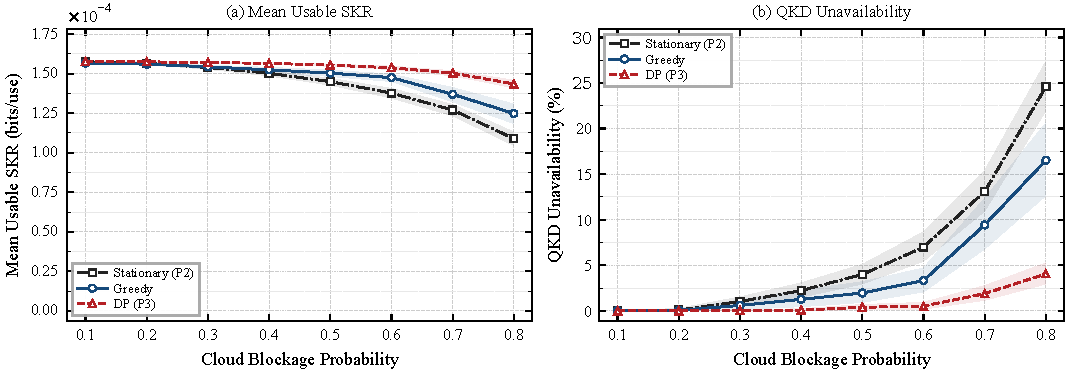
\includegraphics[width=\textwidth]{figures/fig2_cloud_blockage.pdf}
\caption{Cloud blockage sensitivity at $\lambda_{\rm ref}$: (a) mean usable
rate; (b) zero-rate unavailability. Stationary, Greedy, and DP share 100
paired missions; bands are pointwise 95\% whole-mission bootstrap intervals.}
\label{fig:cloud}
\end{figure*}

\section{Numerical Results and Discussion}
\label{sec:numerical}
Table~\ref{tab:parameters} gives the synthetic baseline; cell centers are
$50,150,\ldots,950$ m per axis. Gaussian-copula clouds use spatial covariance
$\exp(-d_{i,j}/\ell)$ and latent AR(1) coefficient $\rho$. Comparisons share
100 mission IDs (0--99); uncertainty uses saved whole-mission bootstrap
intervals. Availability means $S>0$, without an engineering threshold.
The presentation follows~\cite{gong2020}.

\begin{table}[!t]
\caption{Synthetic Baseline and Recorded Optical Parameters}
\label{tab:parameters}
\centering
\begin{tabular}{@{}ll@{}}
\toprule
Parameter & Value\\
\midrule
HAP / UAV altitude & 20 / 1 km\\
HAP horizontal position & $(11419.6551,450)$ m\\
Flight region / candidates & $1\times1$ km$^2$ / 100\\
Mission slots / slot duration & 30 / 20 s\\
$v_{\max}$ / $D_{\rm ref}$ & 15 m/s / 1000 m\\
Cloud $(p,\ell,\rho)$ & $(0.4,250\,\mathrm m,0.9)$\\
Paired missions / seed & 100 / 20261015\\
Exact source catalog & 197 MB + 36 Uniform\\
Wavelength / full divergence & 1550 nm / $233\,\mu$rad\\
Receiver diameter / $\tau_{\rm zen}$ & 0.08 m / 0.92\\
$\beta_{\rm rec}$ / $\xi_{\rm ch}$ & 0.95 / 0.0186 SNU\\
Detector efficiency / noise & 1 / 0\\
$\lambda_{\rm ref}$ (bit/use) & $9.468026677248516\!\times\!10^{-6}$\\
\bottomrule
\end{tabular}
\end{table}

Fig.~\ref{fig:cloud} compares the positioning schemes as blockage increases.
Observed usable rates decrease, but movement can avoid blocked locations.
At $p=0.8$,
mean zero-rate unavailability is 24.60\%, 16.53\%, and 4.07\% for Stationary,
Greedy, and DP, respectively. This availability benefit is observed;
P3 optimizes $U$, not positive-rate slot count.

\begin{figure*}[!t]
\centering
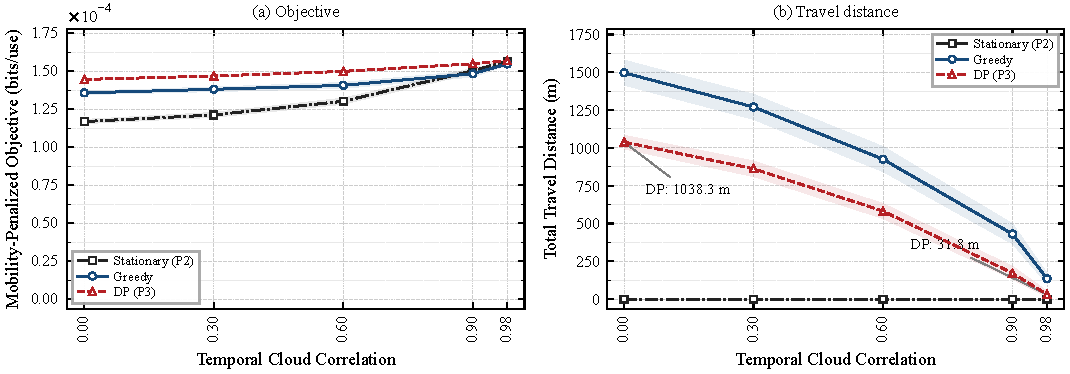
\includegraphics[width=\textwidth]{figures/fig3_temporal_correlation.pdf}
\caption{Latent temporal correlation at $p=0.4$, $\ell=250$ m, and
$\lambda_{\rm ref}$: (a) mean objective; (b) total travel distance.
Methods share 100 mission IDs; bands are pointwise 95\% whole-mission
bootstrap intervals. Latent $\rho$ differs from binary cloud correlation.}
\label{fig:temporal}
\end{figure*}

Fig.~\ref{fig:temporal} shows persistent favorable locations making offline
stationary selection competitive. As $\rho$ increases from
0 to 0.98, mean DP distance falls from 1038.25 to 31.84 m, while its mean
objective gain over P2 falls from 23.712\% to 0.155\%. This sampled trend
is not a correlation monotonicity theorem or an online result. Enlarging
nested position sets, however, cannot lower optimal P2/DP $U$: increasing
$J$ from 10 to 100 improves mean DP $U$ by 11.409\%.

At the default configuration and $\lambda_{\rm ref}$, DP improves mean
usable rate by 4.16\% over P2 and 2.70\% over Greedy, and mean objective
by 3.07\% and 4.42\%, respectively. Relative to zero-penalty DP, the
representative penalty reduces mean travel by 88.370\% with only a 0.515\%
decrease in mean usable rate. All locations select the same
MB source $(\nu,V_A)=(0.125,8)$ at the catalog boundary; these gains
do not isolate shaping gain. Rates retain the security limitations of
Section~\ref{sec:security}; finite-key, tracking, and nonideal-detector
effects~\cite{usenko2016} are excluded.

\section{Conclusion}
\label{sec:conclusion}
Finite-catalog MB source selection and cloud-aware positioning were
compared through Stationary, current-slot Greedy, and offline DP.
DP optimizes the finite-grid penalized objective, with observed blockage
avoidance and a favorable rate--distance tradeoff. Findings remain
conditional on synthetic clouds, offline information, and a distance-cost
surrogate. The two-dimensional MI and homodyne-conditioned Holevo
expressions are not measurement-consistent; a consistent security model
is required before these numerical rates can represent secure keys.

% Generated by IEEEtran.bst, version: 1.14 (2015/08/26)
\begin{thebibliography}{1}
\providecommand{\url}[1]{#1}
\csname url@samestyle\endcsname
\providecommand{\newblock}{\relax}
\providecommand{\bibinfo}[2]{#2}
\providecommand{\BIBentrySTDinterwordspacing}{\spaceskip=0pt\relax}
\providecommand{\BIBentryALTinterwordstretchfactor}{4}
\providecommand{\BIBentryALTinterwordspacing}{\spaceskip=\fontdimen2\font plus
\BIBentryALTinterwordstretchfactor\fontdimen3\font minus
  \fontdimen4\font\relax}
\providecommand{\BIBforeignlanguage}[2]{{%
\expandafter\ifx\csname l@#1\endcsname\relax
\typeout{** WARNING: IEEEtran.bst: No hyphenation pattern has been}%
\typeout{** loaded for the language `#1'. Using the pattern for}%
\typeout{** the default language instead.}%
\else
\language=\csname l@#1\endcsname
\fi
#2}}
\providecommand{\BIBdecl}{\relax}
\BIBdecl

\bibitem{usenko2012}
V.~C. Usenko, B.~Heim, C.~Peuntinger, C.~Wittmann, C.~Marquardt, G.~Leuchs, and
  R.~Filip, ``Entanglement of gaussian states and the applicability to quantum
  key distribution over fading channels,'' \emph{New Journal of Physics},
  vol.~14, p. 093048, 2012.

\bibitem{denys2021}
A.~Denys, P.~Brown, and A.~Leverrier, ``Explicit asymptotic secret key rate of
  continuous-variable quantum key distribution with an arbitrary modulation,''
  \emph{Quantum}, vol.~5, p. 540, 2021.

\bibitem{gong2020}
S.~Gong, H.~Shen, K.~Zhao, R.~Wang, X.~Zhang, T.~de~Cola, and J.~A. Fraire,
  ``Network availability maximization for free-space optical satellite
  communications,'' \emph{IEEE Wireless Communications Letters}, vol.~9, no.~3,
  pp. 411--415, 2020.

\bibitem{usenko2016}
V.~C. Usenko and R.~Filip, ``Trusted noise in continuous-variable quantum key
  distribution: A threat and a defense,'' \emph{Entropy}, vol.~18, no.~1,
  p.~20, 2016.

\end{thebibliography}

\end{document}
